% TO DO: add citations in thesis work, better research plan

\documentclass[10pt]{beamer}
\usetheme[height=0mm]{Rochester}
\usecolortheme{}
\usefonttheme[onlylarge]{structurebold}
\setbeamerfont*{frametitle}{size=\normalsize,series=\bfseries}
\setbeamertemplate{navigation symbols}{}
\setbeamercovered{dynamic}
\setbeamertemplate{itemize item}[triangle]
\setbeamertemplate{itemize subitem}[triangle]

%  use Darmstadt if commenting the next line
\usepackage[footheight=1em]{beamerthemeboxes}
\usepackage[natbib=true,backend=biber,citestyle=authoryear]{biblatex}
\bibliography{../notes/references_gen}

\usepackage{amsmath,amssymb,amsthm,bbm}             % AMS Math
\usepackage[utf8]{inputenc}
\usepackage[english]{babel}
\usepackage{xcolor}
\usepackage{xargs}
\usepackage{graphicx}
\usepackage{subfigure}
\usepackage{hyperref}
\usepackage{mathtools}
\usepackage{mathrsfs}
\def\youngfun{\psi}
\def\htcoeff{\beta}
\def\paramcond{\vartheta}
\def\paramprior{\alpha}
\def\paramvi{\phi}
\def\param{\theta}
\def\paramset{\varTheta}
\def\gauss{\mathcal{N}}
\def\gendim{d_{\epsilon}}
\def\abscont{\ll}
\newcommand{\borel}[1]{\mathcal{B}(#1)}
\newcommand{\mset}[1]{\mathrm{M}_{#1}}
\newcommand{\mxset}[2]{\mathrm{M}(#1, #2)}
\newcommand{\pset}[1]{\mathcal{P}_{#1}}
\providecommand{\alt}[1]{{#1}^{'}}
\newcommand{\tmin}[1]{{#1}^{*}}
\newcommand{\emin}[1]{\hat{#1}}
\newcommand{\youngfunht}[1]{\youngfun_{#1}^{\operatorname{HT}}}
\newcommand{\youngfunc}[1]{\youngfun_{#1}}
\newcommand{\onorm}[2]{\left\|#1\right\|_{#2}}
\newcommand{\kl}[2]{\operatorname{D}_{\operatorname{KL}}\left(#1||#2\right)}
\newcommand{\dist}[2]{\operatorname{D}\left(#1||#2\right)}
\newcommand{\dens}[2]{#1\left(#2\right)}
\newcommand{\condd}[3]{\dens{#1}{#3 | #2}}
\newcommand{\utility}[1]{\mathrm{U}(#1)}
\newcommand{\decfunset}[1]{\mathrm{D}(#1)}
\def\xsp{\mathcal{X}}
\def\gendist{\lambda}
\def\decfun{\delta}
\def\distset{{\pset{}}_{\mathrm{D}}}
\def\stateset{\mathcal{S}}
\def\actionset{\mathcal{A}}
\def\rewardset{\mathcal{Z}}
\def\PP{\mathbb{P}}
\def\rset{\mathbb{R}}
\def\rsetpos{\rset_*}
\def\nsetpos{\mathbb{N}_*}
\def\statesp{\left(\Omega, \mathcal{F}, \PP\right)}
\def\statedim{{d_x}}
\def\latdim{{d_z}}
\def\dataset{\mathcal{D}}
\def\pdata{p_{\dataset}}
\def\ndata{n}
\def\outcomeset{\mathcal{O}}
\def\tensprod{\otimes}
\newcommandx{\wpdist}[3][1=1]{\operatorname{W}_{#1}(#2, #3)}
\newcommand{\dirac}[1]{\delta_{#1}}
\newcommandx\pgen[1][1=\param]{p_{#1}}
\newcommandx{\pgend}[2][1=\param]{\dens{\pgen[#1]}{#2}}
\newcommandx{\empmeas}[1][1=\chunk{\state}{1}{\ndata}]{\mu_{\operatorname{emp}}(#1)}
\newcommand{\chunk}[3]{{#1}_{#2:#3}}
\newcommand{\pdatad}[1]{\dens{\pdata}{#1}}
\newcommandx{\pcond}[1][1=\paramcond]{p_{#1}}
\newcommandx{\pcondd}[3][1=\paramcond]{\condd{\pcond[#1]}{#2}{#3}}
\newcommandx{\pprior}[1][1=\paramprior]{\pi_{#1}}
\newcommandx{\ppriord}[2][1=\paramprior]{\dens{\pprior[#1]}{#2}}
\newcommandx{\pvi}[1][1=\paramvi]{q_{#1}}
\newcommandx{\pvid}[3][1=\paramvi]{\condd{\pvi[#1]}{#2}{#3}}
\newcommandx\pvae[1][1=\param]{p_{#1, \operatorname{full}}}
\newcommandx{\pvaed}[2][1=\param]{\dens{\pvae[#1]}{#2}}
\newcommandx\ppost[1][1=\param]{p_{#1, \operatorname{post}}}
\newcommandx{\ppostd}[3][1=\param]{\condd{\ppost[#1]}{#2}{#3}}
\newcommandx{\dloss}[1]{L(#1)}
\newcommandx{\mloss}[3][3=\lstate]{m(#1, #2; #3)}
\newcommandx{\dmloss}[3][3=\lstate]{g(#1, #2; #3)}
\newcommandx{\empmloss}[3][3=\chunk{\state}{1}{\ndata}]{M_{n}(#1, #2; #3)}
\newcommandx{\tmloss}[2]{M^{\star}(#1, #2)}
\newcommandx{\lpnorm}[3][1=2,2=\pdata]{\left\|#3\right\|_{L^{#1}(#2)}}
\newcommandx{\erisk}[2]{R(#1, #2)}
\newcommand{\m}[1]{\mathrm{#1}}
\newcommand{\lpsp}[2]{\operatorname{L}^{#1}(#2)}
\def\suplogratio{\gamma_r}
\def\supklpost{\gamma_{\operatorname{kl}}}
\def\state{X}
\def\constlogr{c_{r}}
\def\constkl{c_{\operatorname{kl}}}
\newcommand{\PE}[2]{\mathbb{E}_{#1}\left[#2\right]}
\newcommand{\PV}[2]{\mathbb{V}_{#1}\left[#2\right]}
\def\rmd{\mathrm{d}}
\def\eqdef{:=}
\def\eqsp{\;}
\newcommand{\gammafun}[2]{\Gamma(#1; #2)}
\newcommand{\nofrac}[2]{#1 \bigg/ #2}
\newcommand{\indi}[1]{\mathrm{1}_{#1}}
\newcommand{\vfam}[1]{\mathcal{F}(#1)}
\newcommand{\cpl}[2]{\mathcal{C}(#1, #2)}
\def\lstate{x}
\def\bigO{\mathcal{O}}
\newcommand{\jac}[1]{\mathrm{J}_{#1}}
\newcommand{\nflow}[1]{T_{#1}}
\newcommand{\nflowlayer}[1]{\mathcal{T}_{#1}}
\newcommandx{\elbo}[3][1=\paramcond, 2=\paramvi]{m(#1, #2; #3)}
\def\idm{\mathrm{I}}
\usepackage{url}

\definecolor{bleu}{rgb}{0.2,0.4,0.65}
\setbeamercolor{palette primary}{bg=bleu,fg=white}
\setbeamercolor{palette secondary}{bg=bleu,fg=white}
\setbeamercolor{palette tertiary}{bg=bleu,fg=white}
\setbeamercolor{palette quaternary}{bg=bleu,fg=white}
\setbeamercolor{structure}{fg=bleu} % itemize, enumerate, etc
\setbeamercolor{section in toc}{fg=bleu} % TOC sections
\def\figdir{Figures}

\setbeamertemplate{footline}[frame number]

\AtBeginSection[] % Do nothing for \section*
{
\begin{frame}
\frametitle{Outline}
\tableofcontents[currentsection]
\end{frame}
}

\newcommand{\backupbegin}{
   \newcounter{framenumberappendix}
   \setcounter{framenumberappendix}{\value{framenumber}}
}
\newcommand{\backupend}{
   \addtocounter{framenumberappendix}{-\value{framenumber}}
   \addtocounter{framenumber}{\value{framenumberappendix}}
}
\makeatletter


\title[Bayesian ML: Generative Models]{BML lecture \#6: Generative models}
\subtitle{\url{http://github.com/rbardenet/bml-course}}
\author[Gabriel V Cardoso (Mines PSL)] % (optional, for multiple authors)
{Gabriel V Cardoso\\ \url{gabriel.victorino_cardoso@minesparis.psl.eu}}
\institute[] % (optional)
{
  Ecole des Mines, Univ. PSL, France\\
\vspace{1cm}

\includegraphics[width=0.5\textwidth]{figures_gabriel/logo.png}
}
\date{}

\begin{document}
\begin{frame}
\maketitle
\end{frame}

\begin{frame}{Generative models and Bayesian ML: Outline}
  \begin{itemize}
    \item Part I (today): Learning generative models and decision theory.
    \item Part II (next week): Using generative models to solve (Bayesian) inverse problems.
  \end{itemize}
\end{frame}
\begin{frame}{Learning generative models: A "frequentist" approach?}
  \begin{minipage}{0.6\textwidth}
    \pause
    "Frankly, I am not a Bayesian. I go under the following principle. If you don’t understand a problem from a Bayesian decision theory point of view, you don’t understand the problem and trying to solve it is like shooting at a target in the dark. Once you understand the problem, it is not necessary to attack it from a Bayesian point of view. Bayesian methods always had the difficulty that our approximations to our subjective beliefs could carry a lot more information than we thought or felt willing to assume."
  \end{minipage}
  \hspace{5pt}
  \begin{minipage}{0.3\textwidth}
    \begin{flushright}
      \begin{figure}
        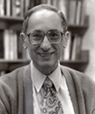
\includegraphics[width=.9\textwidth]{figures_gabriel/chernoff_herman.jpg}
      \end{figure}
    \end{flushright}
  \end{minipage}
\end{frame}
\begin{frame}{Generative modelling as a decision problem: V1}
  \begin{itemize}
    \setlength\itemsep{1.5em}
    \item $\stateset = $:
    \item $\rewardset = $:
    \item $\actionset = $:
    \item "Prior":
    \item SEU:
    \item Bayes action:
  \end{itemize}
\end{frame}
\begin{frame}{Generative modelling as a decision problem: V2}
  \begin{itemize}
    \setlength\itemsep{1.5em}
    \item $\stateset = $:
    \item $\rewardset = $:
    \item $\actionset = $:
    \item "Prior":
    \item SEU:
    \item Bayes action:
  \end{itemize}
\end{frame}
\begin{frame}{"Quasi-Bayes" or Asymptotically Bayes}

\end{frame}
\begin{frame}{Finding Bayes actions: Normalizing flow}
  Let $Z \sim \lambda$ and $\state \sim \nflow{\param}(Z)$. Denote by $\pgen{}$ the law of $\state$.
  \pause

  If $\nflow{\param}$ is an invertible map for all $\param$, then
  \begin{equation}
      \pgen(\lstate) = \gendist(\nflow{\param}^{-1}(\lstate))\left|\det \jac{\nflow{\param}}(\nflow{\param}^{-1}(\lstate))\right| \eqsp.
  \end{equation}
  \pause

  A normalizing flow is defined by
  \begin{equation}
      \label{eq:nflow_def}
      \nflow{\param}: \lstate \in \xsp \rightarrow \nflowlayer{\param_k}\circ \cdots \circ \nflowlayer{\param_0}(\lstate) \in \xsp \eqsp,
  \end{equation}
  where each $\nflowlayer{\param_k}: \xsp \rightarrow \xsp$ is an invertible map with \textbf{easy} to compute Jacobian determinants.   
\end{frame}
\begin{frame}{Finding Bayes actions: Normalizing flow}

  A typical example of such flow is the RealNVP \citep{dinh2017density}, defined as:
  \begin{equation}
      \label{eq:rnvp_def}
      \nflowlayer{\param}(\lstate[1{:}d], \lstate[d{:}\statedim]) = (\lstate[1{:}d], \lstate[d{:}\statedim] \cdot e^{s(\lstate[1{:}d]; \param)} + t(\lstate[1{:}d]; \param)) \eqsp,
  \end{equation}
  where $s(\cdot; \param), t(\cdot; \param): \rset^d \rightarrow \rset^{\statedim - d}$ are typically neural networks.
  
  The Jacobian of such flow is
  \begin{equation}
      \label{eq:rnvp_jac}
      \jac{\nflowlayer{\param}}(\lstate) = \begin{bmatrix}
          \idm{d} & 0 \\
          \cdots & \operatorname{diag}(e^{s(\lstate[1{:}d]; \param)})
      \end{bmatrix}\eqsp,
  \end{equation}
  and thus $\det \jac{\nflowlayer{\param}}(\lstate) = e^{\sum_{j=1}^{\statedim - d} s(\lstate[1{:}d]; \param)[j]}$.
\end{frame}
\begin{frame}{Proving quasi-Bayes: A toy proof}
  \vspace{-100pt}
  Suppose that
  \begin{itemize}
    \item $\xsp$ is compact, $\paramset$ is compact and
    \item $\nflow{\param}$ is continuous.
  \end{itemize}

  Can we prove that with high probability
  \begin{equation}
    \lim_{\ndata \rightarrow \infty} \PE{\pdata}{\log \pgen[\decfun_n(\chunk{\state}{1}{n})](\state)}- \PE{\pdata}{\log \pgen[\tmin{\decfun}](\state)} = 0 \eqsp ?
  \end{equation}
\end{frame}
\begin{frame}{Proving quasi-Bayes: A toy proof}
  
\end{frame}
\begin{frame}{Why we care: The Cournot's principle.}
  \begin{minipage}{0.6\textwidth}
    \pause
    "$\cdots$ The physically impossible event is therefore the one that has infinitely small probability, and only this remark gives substance—
objective and phenomenal value—to the theory of mathematical
probability.

\hspace{2pt}

$\cdots$ L’événement physiquement impossible est donc celui dont la prob-
abilité mathématique est infiniment petite; et cette seule remarque
donne une consistance, une valeur objective et phénomènale à la
théorie de la probabilité mathématique." \footnote{Taken from \fullcite{shaferthats} which is itself a citation of Cournot's original work.}
  \end{minipage}
  \hspace{5pt}
  \begin{minipage}{0.3\textwidth}
    \begin{flushright}
      \begin{figure}
        \includegraphics[width=.9\textwidth]{figures_gabriel/Antoine_Augustin_Cournot.jpg}
      \end{figure}
    \end{flushright}
  \end{minipage}
\end{frame}
\begin{frame}{Duality and The latent model}
  \vspace{-95pt}
  \begin{theorem}[\cite{donsker1983asymptotic}]
    Let $(q, p) \in \pset{}$, such that $p \abscont q$ and $q \abscont p$. Then, 
    \begin{equation}
        \kl{q}{p} = \sup_{f \in \mathcal{G}_{q}} \PE{q}{f} - \log \PE{p}{\exp(f)} \eqsp,
    \end{equation}
    where $\mathcal{G}_q$ is the set of measurable $g$ such that $\PE{q}{\exp(g)} < \infty$.
    Furthermore, equality hold if and only if $f = \log \frac{\rmd q}{\rmd p}$.
  \end{theorem}
\end{frame}
\begin{frame}{Duality and the latent model}

\end{frame}
\begin{frame}{Generative modelling as a decision problem: The VAE case}
  \begin{itemize}
    \setlength\itemsep{1.5em}
    \item $\stateset = $:
    \item $\rewardset = $:
    \item $\actionset = $:
    \item "Prior":
    \item SEU:
    \item Bayes action:
  \end{itemize}
\end{frame}
\begin{frame}{Proving quasi-Bayes: Going further}
  \begin{flushright}
    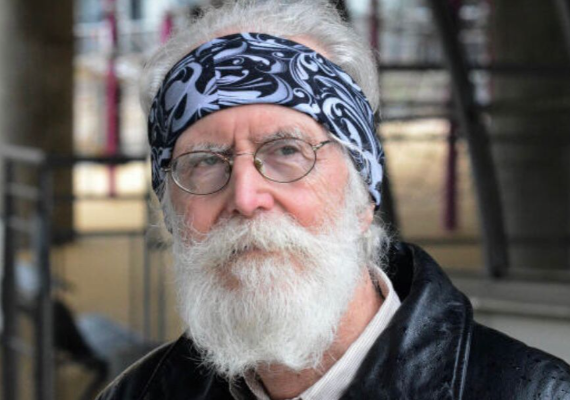
\includegraphics[width=0.3\textwidth]{figures_gabriel/talagrand.png}
  \end{flushright}
\end{frame}
\begin{frame}{Proving quasi-Bayes: the VAE case}
  \begin{theorem}[{\cite{tang2021empirical}[Theorem 3]}]
      Define $\decfun_n(\chunk{\lstate}{1}{n}) = (\emin{\paramcond}, \emin{\paramvi})$ and $\tmin{\decfun} = (\tmin{\paramcond}, \tmin{\paramvi})$. Suppose that the parameter space is compact and that 
      for all $\lstate \in \xsp$,
      \begin{equation*}
        |\elbo{\lstate} - \elbo[\tilde{\paramcond}][\tilde{\paramvi}]{\lstate} | \leq b(\lstate) \|(\paramcond, \paramvi) - (\tilde{\paramcond}, \tilde{\paramvi}) \| \eqsp,
      \end{equation*}
      with $\PE{}{b^2(\state)} < \infty$. Then, under additional hypothesis\footnote{Control of the Orlicz norm of the r.v. $\elbo{\state}$ uniformly on the parameter. See \cite{tang2021empirical}[Assumption A].}, the event
      \begin{align*}
        \PE{\pdata}{\elbo[\emin{\paramcond}][\emin{\paramvi}]{\state}} \leq &\inf_{\eta}\left\{(1+\eta)\PE{\pdata}{\elbo[\tmin{\paramcond}][\tmin{\paramvi}]{\state}} \right. \\
        &\left.+ c_2(1 + \eta^{-1})\frac{Dd_{\param}}{\ndata}\log(\ndata d_\param)\log^{\frac{1}{\alpha}}\ndata\right\} \eqsp,
      \end{align*}
      happens with probability $1 - c_0 \exp(-c_1 \left(d_\param \log \ndata\right)^{\min\{\alpha, 1\}})$. 
  \end{theorem}
\end{frame}

\begin{frame}{Generative modelling as a decision problem: The Wasserstein case}
  \begin{itemize}
    \setlength\itemsep{1.5em}
    \item $\stateset = $:
    \item $\rewardset = $:
    \item $\actionset = $:
    \item "Prior":
    \item SEU:
    \item Bayes action:
  \end{itemize}
\end{frame}
\begin{frame}{Wasserstein / KL link}
  \begin{flushright}
    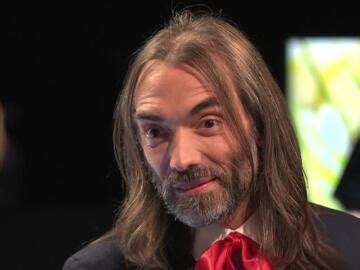
\includegraphics[width=0.3\textwidth]{figures_gabriel/villani.jpeg}
  \end{flushright}
\end{frame}
\begin{frame}{Proving quasi-Bayes: The WGAN case \cite{biau2021theoretical}}
  \begin{theorem}[{\cite{biau2021theoretical}[Theorem 21]}]
    Assume the parameter space is compact\footnote{See Assumption 1 of \cite{biau2021theoretical} for a precise definition.} and define for $\mathcal{D} \subset \rset^{\xsp}$ 
    \begin{equation}
      d_{\mathcal{D}}(\mu, \nu) \eqdef \sup_{D \in \mathcal{D}} {\PE{\mu}{D} - \PE{\nu}{D}} \eqsp.
    \end{equation}
    For any $\epsilon > 0$ and $\eta \in (0, 1)$,  there exists $\mathcal{D}$ ($\mathcal{D}(\epsilon)$), such that for
    \begin{itemize}
      \item ${\pdata}$ \textbf{compact with diameter} $B$,
        the event 
        \begin{equation*}
          d_{\mathcal{D}}(\pdata, \pgen[\decfun_n(\chunk{\state}{1}{n})]{}) - d_{\mathcal{D}}(\pdata, \pgen[\tmin{\decfun}]{}) \leq 2\epsilon + \frac{c_1}{\sqrt{\ndata}} + B \sqrt{\frac{\log(1/\eta)}{2\ndata}}
        \end{equation*}
      \item ${\pdata}$ \textbf{$\gamma$ sub-Gaussian,} the event
        \begin{equation*}
          d_{\mathcal{D}}(\pdata, \pgen[\decfun_n(\chunk{\state}{1}{n})]{}) - d_{\mathcal{D}}(\pdata, \pgen[\tmin{\decfun}]{}) \leq 2\epsilon + \frac{c_2}{\sqrt{\ndata}} + 8\gamma \sqrt{e \statedim}\sqrt{\frac{\log(1/\eta)}{2\ndata}}
        \end{equation*}
    \end{itemize}
    happens with probability $1 - \eta$.
  \end{theorem}
\end{frame}
\begin{frame}{$\stateset = \xsp^{n} \times \paramset$ anyone?}

\end{frame}
\begin{frame}{Statisticians produce knowledge vs Statistician produces solutions}
  \begin{minipage}{0.6\textwidth}
    \pause
    "Unfortunately, our field has a vested interest in data models, come hell or high water. 
     For instance, see Dempster’s (1998) paper on modeling.
     His position on the 1990 Census adjustment controversy is particularly interesting.
     He admits that he doesn’t know much about the data or the details, but argues that the problem can be solved by a strong dose of modeling.
     That more modeling can make error ridden data accurate seems highly unlikely to me.
     Terrabytes of data are pouring into computers from many sources, both scientific, and commercial, and there is a need to analyze and understand the data.
     $\cdots$ This is a fascinating enterprise, and I doubt if data models are applicable.
     Yet I would enter this in my ledger as a statistical problem." \footfullcite{breiman2001statistical}.
  \end{minipage}
  \hspace{10pt}
  \begin{minipage}{0.25\textwidth}
    \begin{flushright}
      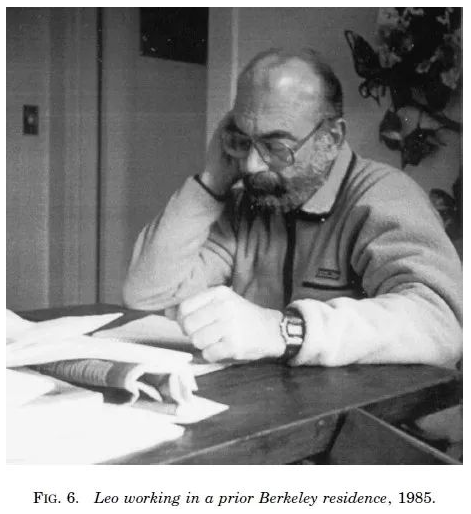
\includegraphics[width=1\textwidth]{figures_gabriel/leo_breiman.png}
    \end{flushright}  
  \end{minipage}
\end{frame}
\begin{frame}{Back to Savage}
  "For an example, suppose your roommate is to decide between two bets: bet
  (i) gives \$5 if Duke and not UNC wins this year's NCAA final, and \$0
  otherwise; $\cdots$ you can ask your roommate whether he or she would prefer lottery (i) to (iii), where you win $0$ if Duke wins this year’s NCAA championship, and you win $5$ otherwise.
   If your roommate is indifferent then it has to be that he or she considers Duke winning and not winning to be equally likely.
  "\footfullcite[Chapter 5]{parmigiani1997decision}
\end{frame}
\begin{frame}{Working towards $\stateset = \xsp^{n} \times \paramset$}
  \fullcite{papamarkou2024position}
\end{frame}
\begin{frame}{Extra: PAC-Bayes}
  \begin{itemize}
    \setlength\itemsep{1.5em}
    \item $\stateset = $:
    \item $\rewardset = $:
    \item $\actionset = $:
    \item "Prior":
    \item SEU:
    \item Bayes action:
  \end{itemize}
\end{frame}
\begin{frame}{Extra: PAC-Bayes}
  \begin{itemize}
    \item \textbf{Compactness of the data:} $\xsp$ is a compact set
    \item \textbf{Lipschitzness of the decoder:} $\mathcal{K}(\xsp; \pset{\pprior}) = \{\lstate \in \xsp \rightarrow \gauss(\mu_q(x), \Sigma_q(x)) \}$, and for $q \in \mathcal{K}(\xsp; \pset{\pprior})$, the functions $m_q(x), \Sigma_q(x)$ are both $K_{q}$-Lipschitz.
    \item \textbf{Lipschitzness of the encoder:}The function $z \in \rset^{\latdim} \rightarrow \log \pgen(\lstate|z)$ is $K_{\param}$-Lipschitz for all $\lstate$.
\end{itemize}
\begin{theorem}[Reconstruction bound (Theorem 4.3 from \cite{mbacke2023statistical})]
    \label{thm:gen:vae:rec_bound}
    Let $\Delta = \sup_{(\lstate, \tilde{\lstate}) \in \xsp^2} \|\lstate - \tilde{\lstate}\|$. For any $\param \in \paramset$, $\delta > 0$, $\lambda > 0$, with probability at least as high as $1 - \delta$,
    \begin{align}
        &\PE{\pdata}{\PE{q(\cdot | \state)}{ - \log \pgen[\param](\state | Z)}} \leq \PE{\empmeas}{\PE{q(\cdot | \state)}{ - \log \pgen[\param](\state | Z)}} \\
        &+ \lambda^{-1}\left[\PE{\empmeas}{\kl{q(\cdot|\state)}{\pprior}} + \lambda K_{q} K_{\param}\Delta + n^{-1}\log \left({1}/{\delta}\right) + \frac{\lambda^2 \Delta^2}{8} \right] \eqsp.
    \end{align}
\end{theorem}
\end{frame}
\begin{frame}{Generative prior in Bayesian statistics: Likelihood free}

\end{frame}
\begin{frame}{Inverse problems}

\begin{equation*}
    Y = A \state + \sigma_y Z \eqsp,
\end{equation*}
where $A \in \mxset{d_y}{\statedim}$, $Z \sim \gauss(0, \idm_{d_y})$ and $\sigma_y > 0$. 

\begin{figure}[h!]
    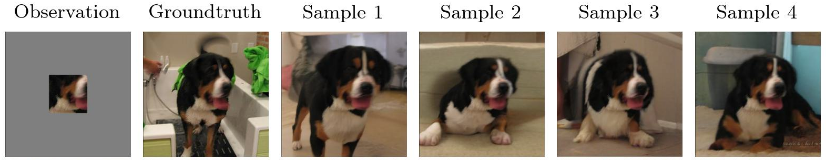
\includegraphics[width=\textwidth]{../notes/images_gabriel/example_inpainting_yazid.png}
    \caption{Figure taken from \cite{moufad2024variational}. The "Observation" corresponds to $y$ that was obtained with the ground truth $\state$. The other columns correspond to solutions of a certain inverse problem.}
\end{figure}
\end{frame}
\begin{frame}{Generative prior in Bayesian statistics: Inverse problems}
    You are an environmental agent and you should decide to authorize or not the drilling in a certain region.
    You have to determine if the drilling of the region affects the water resources of the region.
    The only information you have is the drilling profiles for certain wells, as in \ref{fig:flummy_example}, which we denote by $y$.
    Let denote by $A$ the event corresponding to the fact that there is an underground channel passing through $A$.
  \begin{figure}[h!]
    \centering
    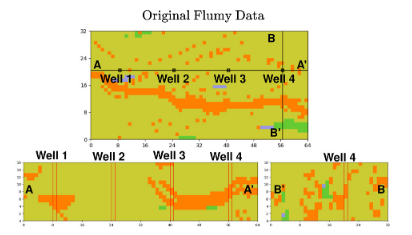
\includegraphics[width=0.6\textwidth]{../notes/images_gabriel/example_flummy.png}
    \label{fig:flummy_example}
    \caption{Figure taken from \cite{bhavsar2023principled}.}
  \end{figure}
\end{frame}
\begin{frame}{Bayesian inverse problems as a decision problem}
  \begin{itemize}
    \setlength\itemsep{1.5em}
    \item $\stateset = $:
    \item $\rewardset = $:
    \item $\actionset = $:
    \item "Prior":
    \item SEU:
    \item Bayes action:
  \end{itemize}
\end{frame}
\section*{References}
\setbeamertemplate{bibliography item}[text]%,
\begin{frame}[allowframebreaks]
\frametitle{References}
\small
\printbibliography
\normalsize
\end{frame}

\end{document}